\documentclass{ximera}
\graphicspath{
{./}
{volumes/}
{arclengths/}
{centroids/}
{techniques/}
{applications/}
{series/}
{powerseries/}
{odes/}
{lessons/}
}
\usepackage{booktabs}

\newcommand{\bigmath}[1]{$\displaystyle #1$}
\newcommand{\choicebreak}{}
\newenvironment{type}{}{}
\newenvironment{notes}{}{}
\newenvironment{keywords}{}{}
\newcommand{\offline}{}
\newenvironment{comments}{\begin{feedback}}{\end{feedback}}
\newenvironment{multiplechoice}{\begin{multipleChoice}}{\end{multipleChoice}}
\title{Exercises: ODE Applications}
%%%%%\author{Philip T. Gressman}

\begin{document}
\begin{abstract}
Exercises relating to the application of ODEs to solve problems.
\end{abstract}
\maketitle



\begin{exercise}
Find the orthogonal trajectories of the given family (represented by the purple curves in the plot below):
\[ y = C e^{-x}. \]
Write your answer as $f(y) = g(x) + C$, where both $f(y)$ and $g(x)$ vanish at the origin. Moreover, you should multiply by constants if necessary so that $f(1) = 1/2$ and $g(1) = 1$. 
\[ \answer{\frac{1}{2} y^2} = \answer{x} + C. \]
\begin{center}
\begin{image}
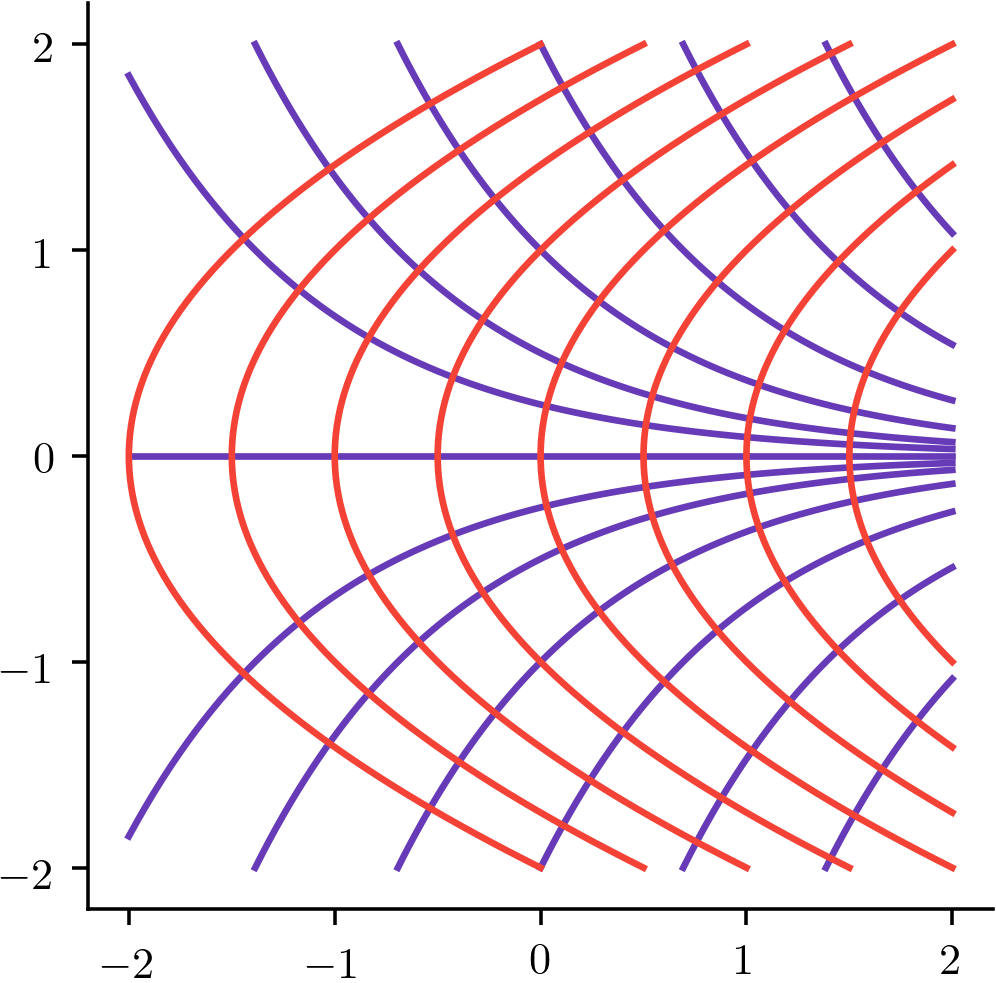
\includegraphics[width=4in]{images/ortho01.png}
\end{image}
\end{center}

\end{exercise}

\begin{exercise}
Find the orthogonal trajectories of the given family (represented by the purple curves in the plot below):
\[ y = x - \frac{x^3}{3} + C. \]
Write your answer as $y = f(x) + C$, where $f(0) = 0$
\[ y = \answer{\frac{1}{2} \ln \left| \frac{1-x}{1+x} \right|} + C. \]
\begin{center}
\begin{image}
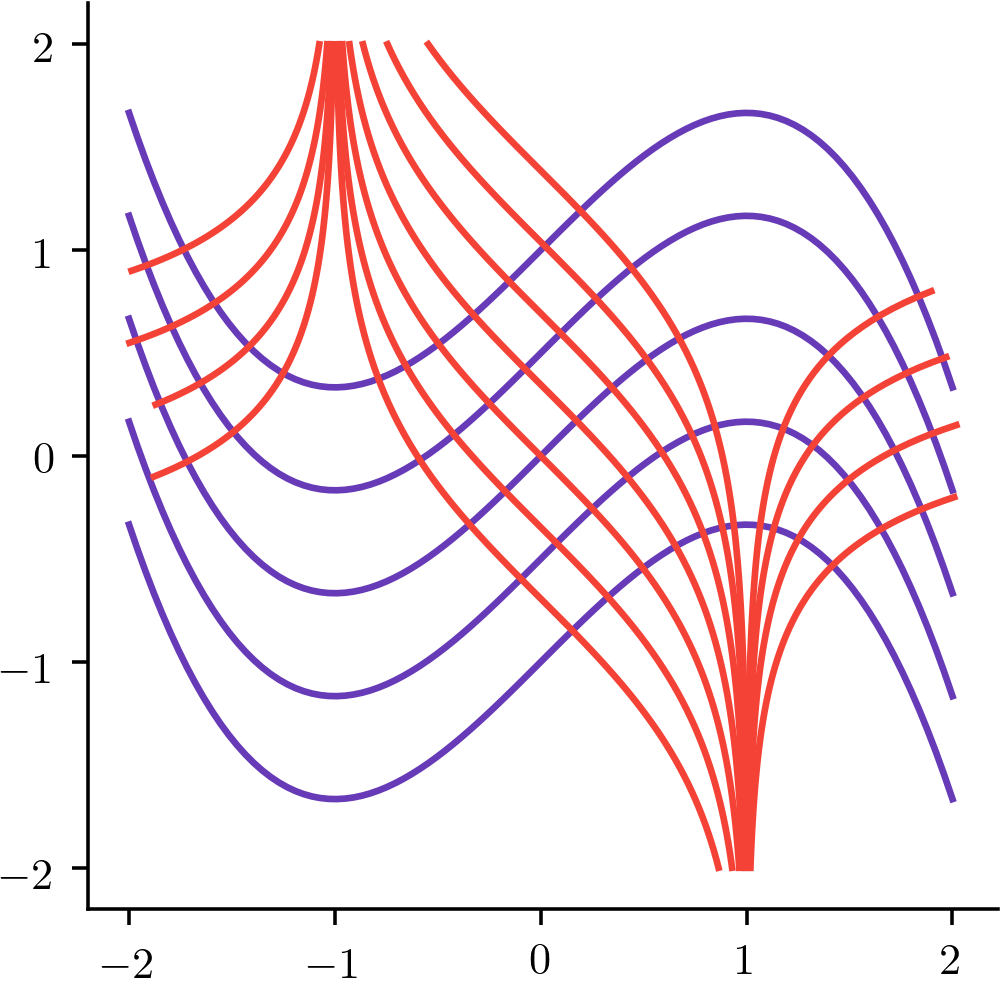
\includegraphics[width=4in]{images/ortho02.png}
\end{image}
\end{center}

\end{exercise}

\begin{exercise}
Find the orthogonal trajectories of the given family:
\[ y = \tan \left( C + x + \frac{x^3}{3} \right) \]
Write your answer as $f(y) = g(x) + C$, where both $f(y)$ and $g(x)$ vanish at the origin. Moreover, you should multiply by constants if necessary so that $f(1) = 4/3$ and $g(1) = -\pi/4$.
\[ \answer{y + \frac{y^3}{3}} = \answer{- \arctan x} + C \]
\end{exercise}



\begin{exercise}
It takes about three days to defrost a 10 pound imitation frozen turkey in a home refrigerator. Suppose that the initial temperature is $-16^\circ$C and the ambient temperature is $2^\circ$C inside the refrigerator. If after exactly two days, the temperature of the frozen turkey is $0^\circ$C, find a formula for the temperature $y(t)$ (in degrees Celsius) as a function of time for all $t > 0$, where $t$ is measured in days
\[ y = \answer{ -18 e^{-t \ln 3} + 2}. \]
\end{exercise}

\begin{exercise}
At time $t = 0$, a cup of tea has temperature $46^\circ$C. Ten minutes later, its temperature is $34^\circ$C. Ten minutes after that, the temperature is then $28^\circ$C. Assuming the temperature obeys Newton's Law of cooling, what is the temperature (in degrees Celsius) as a function of time $y(t)$ for all $t > 0$, where $t$ is measured in minutes?
\[ y(t) = \answer{24 e^{-t \ln(2)/10} + 22}  \]
\begin{hint}
Suppose $A$ is the ambient temperature. We know that
\[ \frac{48-A}{34 - A} = \frac{34 - A}{28 - A} \]
because every ten minutes, the \textit{difference} between tea temperature and room temperature decreases by the same factor.
\end{hint}
\end{exercise}


\begin{exercise}
A 1000 liter tank is filled with a sugar solution: 200 kilograms of sugar dissolved in 1000 liters of pure water. The solution in the tank is kept thoroughly mixed at all times. At time $t = 0$, the attendants begin adding 1 liter per minute of dissolved sugar at a concentration of 0.1 kilograms per liter. At the same time, One liter per minute is drained from the tank to keep the overall volume of solution in the tank at 1000 liters. Find a function $S(t)$ for the total amount of sugar in the tank (in kilograms) a time $t > 0$, where $t$ is measured in minutes.
\[ S(t) = \answer{ 100 + 100 e^{-t/1000}}. \]
\end{exercise}

\begin{exercise}
A small flask contains 10mL of solvent in which 1 gram of substance X is initially dissolved. The solution is slowly drained at a rate of 3mL per hour while 4mL per hour of pure solvent is added (with the whole solution being kept thoroughly mixed). Find a formula $X(t)$ for the amount of substance $X$ (in grams) sill in the beaker at time $t$, where $t$ is measured in hours.
\[ X(t) = \answer{ \frac{1000}{(t+10)^3}}. \]
\end{exercise}



\section*{Sample Exam Questions}

\begin{question}%%%%%[2016C.15]

A tank contains 100 gallons of water in which 300 pounds of salt are dissolved. At some initial time, workers begin pumping in fresh water, i.e., containing no salt, at a rate of 10 gallons per minute. During the process, the tank is kept well-mixed and 20 gallons per minute of the resulting saltwater are pumped out of the tank (in particular, note that the tank will be empty after 10 minutes). Find the total amount of salt in the tank (measured in pounds) which remains 9 minutes after the process starts.
\begin{multiplechoice}
\choice{\(1\)}
\choice{\(2\)}
\choice[correct]{\(3\)}
\choice{\(4\)}
\choice{\(5\)}
\choice{\(6\)}
\end{multiplechoice}

\end{question}


\end{document}
